% !TeX root = document.tex
% !TeX encoding = UTF-8 Unicode

\chapter{Switching Rules}%
\label{chp:switching-rules}

This chapter presents two switching rules: the dwell-time, the most employed and
studied of such techniques in literature, and the proposed rule based on the
region of attraction. Other techniques exist, like using robust control to find
a controller that never makes the system unstable; however, they are more
conservative and not viable in many cases.

\section{Dwell-time}%
\label{sec:dwell-time}

As discussed in Section~\ref{sec:switched-systems}, the act of switching can
cause instability, even if all modes are stable. Although it is possible to
verify if the system is stable under arbitrary switching (and therefore to
design controllers to do so), the procedure is not straight-forward and
challenging to apply to most real-world situations.

There are, however, other ways of verifying and guaranteeing the stability of
systems under switches governed by some rules. The dwell-time is one of such
techniques that restricts the switching signal \(\sigma{}(t)\) to the set
%
\begin{equation}
  \mathcal{D}_{T} := \{\sigma(\cdot):t_{k+1}-t_{k}\ge{}T\},
\end{equation}
%
where \(t_{k}\) and \(t_{k+1}\) are the switching instants, for all
\(k\in{}\mathbb{R}\), which forces the system to remain for \(T\) seconds on a
mode before switching to next one~\parencite{colaneri:dwell}. This is called a
slow switch. The timer is restarted every time the reference changes and
switching is only allowed after \(T\) seconds has passed. For large enough
values of \(T\), this rule guarantees the system's stability.

As the dwell-time certifies stability of the switch, it decouples the switching
logic and the system stability, making it possible to analyse the system
stability for each mode independently. One problem, however, is that computing
the minimum dwell-time is not easy and is the focus of current research. An
easier problem is to find an upper bound for it, which can be done efficiently
using numerical algorithms~\parencite{colaneri:dwell}.

Another technique that uses the concept of dwell-time is the average dwell-time,
where the switching rule \(\sigma\) allows for a fixed number of discontinuities
\(N_{\sigma}(t,\tau)\) for \(t\ge{}\tau{}\ge{}0\) such that the set
\(\mathcal{D}_{T_{D},N_{0}}\) satisfies
%
\begin{equation}
  N_{\sigma}(t,\tau) \le{} N_{0} + \frac{t-\tau}{\tau_{D}},
\end{equation}
%
where \(\tau_{D}\) is the average dwell-time and \(N_{0}\) is the chatter
bound~\parencite{hespanha.morse:stability}. This set is larger than
\(\mathcal{D}_{T}\) and allows for signals with discontinuities separated by at
most \(\tau_{D}\).

To illustrate how the dwell-time works, consider the fictional system if
Figure~\ref{fig:dt-ex1}. The ellipses represent each mode's constraint region,
the black star is the system state, the orange star (in the middle) is the
waypoint and the yellow star the reference. The system will use the dwell-time
rule to switch.

\begin{figure}[!htb]
  \centering
  \includesvg[width=0.5\linewidth]{imgs/dt-ex1}
  \caption{System to be considered in the example}%
  \label{fig:dt-ex1}
\end{figure}

To avoid constraint violation, the reference is first set to the waypoint by the
supervisor. As the reference changed, the timer will be restarted and the system
will only be allowed to change mode after the dwell-time ellapses. However, the
system may fully converge to the waypoint before that, making it just wait,
idle, for the timer to ellapse, as depicted in Figure~\ref{fig:dt-ex2}.

\begin{figure}[!htb]
  \centering
  \includesvg[width=0.5\linewidth]{imgs/dt-ex2}
  \caption{First state's path: convergence to the waypoint}%
  \label{fig:dt-ex2}
\end{figure}

The system will change modes after the timer ellapses and the reference will be
set to the desired reference, in yellow. Because the reference was changed
again, the timer will restart again, with the dwell-time of the second mode.
Figure~\ref{fig:dt-ex3} shows this movement.

\begin{figure}[!htb]
  \centering
  \includesvg[width=0.5\linewidth]{imgs/dt-ex3}
  \caption{Second state's path: convergence to the final reference}%
  \label{fig:dt-ex3}
\end{figure}

As it is the final reference, this timer will not affect the overall
performance, however, if there were more modes to go through, their dwell time
would be summed, and the total convergence time would be at least the sum of all
dwell-times that need to be executed on the path to the final reference.

Algorithm~\ref{alg:dwell-time} formalizes this procedure.

\begin{algorithm}[H]
  \begin{algorithmic}[1]
	\State{}\textbf{Input}: \(\CG{}_i\) \(\leftarrow{}\) current \CG{},~\(\CG{}_j\) \(\leftarrow{}\) target GG.\@
	\State{}change \(r(k)\) to next way-point
	\While{dwell-time of \(\CG{}_{i}\) not ellapsed}
		\State{}calculate \(g(k)\)
		\State{}execute controller
	\EndWhile{}
	\State{}change to \(\CG{}_j\)
	\State{}restart algorithm
  \end{algorithmic}
  \caption{dwell-time implementation}%
  \label{alg:dwell-time}
\end{algorithm}

\section{Region of Attraction}%
\label{sec:roa-switching-rule}

The goal of this switching rule is to allow the system to converge faster to the
final reference when going through a path of restricted mode switches. To do so,
it is necessary to:

\begin{enumerate}
  \item guarantee stability after switching modes,
  \item switch modes as soon as possible.
\end{enumerate}

To guarantee stability, the concept of a controller's region of attraction is
used. As described in Section~\ref{sec:region-of-attraction}, the controller's
region of attraction is a closed region in the state-space such that every
initial state inside it will remain inside it as well as asymptotically converge
to a point inside it (usually the origin of the linearized system).

The region of attraction is, therefore, a certificate of stability for a system.
However, as stated in Section~\ref{sec:switched-systems}, having stable modes is
not enough to guarantee the stability of the system after switching.
Nonetheless, the following region of attraction based rule guarantees that the
system will remain stable after switching:

\begin{align}
  \sigma_{i} = \begin{cases}
    1 & \textrm{if}~f\hat{\xi}_{i}(k)\in\mathcal{L}_V(P_i) \\
    0 & \textrm{otherwise}
  \end{cases},
\end{align}
%
where \(\hat{\xi}_{i}(t)\) is the mode's state, \(\mathcal{L}_V(P_i)\) is the
region of attraction (level set of the \(P_{i}\) matrix from the Lyapunov
function), and \(\sigma_{i}\) is the switching rule, meaning that the system can
switch to the \(i\)th mode if \(\sigma_{i}=1\).

Let us discuss the stability of the system when this rule is used. Suppose a
system is currently in mode 1, and the supervisor has deemed that it needs to go
mode 2. The switch will only occur when the system's state is inside the second
mode's controller's region of attraction. Because it is inside the region of
attraction, it guarantees that it will converge, and therefore the switch is
stable.

Now consider the same scenario, but the mode change follows the path
\(1 \rightarrow 3 \rightarrow 8 \rightarrow 2\), meaning that, to go from \(1\) to \(2\), it first needs to
switch to \(3\), then to \(8\) and only then to \(2\). The worst-case would be
if the system is in the middle of the intersection of all regions of attraction.
In this case, the system will instantly switch modes, going from \(1\) to \(2\)
in \(3\) sample times, in the case of a discrete system. However, since the
switch can only happen when the state is inside the next mode's controller's
region of attraction, it will simply cause the previous scenario to be applied
recursivelly, and the system will remain stable after it reaches the last mode.

In another scenario, the supervisor might malfunction or have a badly defined
rule that will make the reference jump between many values, making the system
try to switch modes seemly randomly. In this case the system will do the
switches as long as it is allowed, but the state will always be inside some
controller's region of attraction. It will then either never converge nor
diverge (because of the ever-changing reference) or enter a state that is only
inside one mode's controller's region of attraction, at which point it will not
switch modes anymore.

The illustrative scenarios show that the state will always be inside some
controller's region of attraction, and therefore it is not possible for the
system to diverge. It can oscilate due to varying references, but that is a case
of malfunction or badly desined referencing system, not normal operation.
Furthermore, when used in conjunction with Command Governors, the reference is
always guaranteed to be inside the region of attraction (since the constraint
region is completely contained inside it), even if the supervisor's reference is
not, eliminating the possible scenario where the system diverges because the
reference is outside the region of attraction, dragging the system out of it.

To visually illustrate the technique, consider the fictional system depicted in
Figure~\ref{fig:roa-ex1}, where the black star is the system's state, the yellow
star is the supervisor's reference, the orange star is the waypoint, the filled
ellipses are the mode's constraints and the circles are the regions of
attraction.

\begin{figure}[!htb]
  \centering
  \includesvg[width=0.45\linewidth]{imgs/roa-ex1}
  \caption{System to be considered in the example}%
  \label{fig:roa-ex1}
\end{figure}

As the system cannot violate constraints, the supervisor will set the reference
to the waypoint, and the system will converge to it. However, as soon as it
crosses the next mode's controller's region of attraction (or after some
distance is travelled inside it, just to be safe), as shown if
Figure~\ref{fig:roa-ex2}, it can switch modes without switching the constraints,
what we call a hybrid switch. This is opitional, but may yield better overall
performance.

\begin{figure}[!htb]
  \centering
  \includesvg[width=0.45\linewidth]{imgs/roa-ex2}
  \caption{System's state crossing the region of attraction's border}%
  \label{fig:roa-ex2}
\end{figure}

The system will then continue to converge to the waypoint, since it can only
change to the next reference once it is inside the constraint's intersection. As
soon as it enters the intersection the full mode change will be performed,
changing the current constraint to that of the next mode and setting the
reference to the global one, represented by the yellow star. Note that the
system does not fully converge to the waypoint. This step is shown in
Figure~\ref{fig:roa-ex3}.

\begin{figure}[!htb]
  \centering
  \includesvg[width=0.45\linewidth]{imgs/roa-ex3}
  \caption{System's state crossing the constraint's intersection's border}%
  \label{fig:roa-ex3}
\end{figure}

With this switching rule, there is no wait: the system will change mode as soon
as possible, yielding faster overall convergence. The hybrid switching is an
addition that may increase the performance of the system at the cost of
computation resources, but is not necessary and can be safelly ignored.
Algorithm~\ref{alg:roa-rule} shows the proposed rule in both its forms, assuming
the use of a Command Governor, which is always recommended for this rule as it
helps to guarantee stability.

\begin{algorithm}[H]
  \begin{algorithmic}[1]
    \State{}\textbf{Input}: \(\CG{}_i\) \(\leftarrow{}\) current \CG{},~\(\CG{}_j\) \(\leftarrow{}\)
        target GG.\@
    \State{}let \(P_1\) and \(P_2\) be regions of attraction for \(\CG{}_i\)
        and \(\CG{}_j\), respectively.
    \If{should switch controllers earlier}
      \While{\(\hat{\xi}(k)\not\in\mathcal{L}_V(P_2)\)}
        \State{}calculate \(g(k)\)
        \State{}execute controller
      \EndWhile{}
      \State{}change current controller and model to \(\CG{}_j\)'s ones
      \State{}reset integrators
    \EndIf{}
    \While{\(x(k)\not\in\mathcal{X}_i\cap\mathcal{X}_j\) or \(\hat{\xi}(k)\not\in\mathcal{L}_V(P_2)\)}
      \State{}calculate \(g(k)\)
      \State{}execute controller
    \EndWhile{}
    \State{}change to \(\CG{}_j\)
    \State{}reset integrators if not already done
    \State{}change \(r(k)\) to next way-point
    \State{}restart algorithm
  \end{algorithmic}
  \caption{Switching rule based on region of attraction}%
  \label{alg:roa-rule}
\end{algorithm}

\section{Practical Implementation Aspects}%
\label{sec:practival-implementation-aspects}

When implementing the techniques described in this thesis, some details need
attention. For example, it is easy to say
\enquote{\(\mathrm{minimize}~f(x)~|~x\in\mathcal{X}\)}, however it is not so
simple (and sometimes even possible) to implement the \(x\in\mathcal{X}\) bit.
Describing the set and finding a way to test membership numerically can be
challenging. That is one reason why we choose convex sets: we know how to
implement membership tests and use it in common optimization frameworks.

This chapter will discuss how to represent the constraints and region of
attraction and provide some insight into how to implement the models of the
command governor with a supervisor structure, and the problems faced when
estimating the region of attraction.

\subsection{Polytope representations}%
\label{subsec:polytope-representation}

A convex polytope can approximate any convex region. A convex polytope is a
compact convex set with a finite number of extreme points such that, for any two
distinct points \((a,b)\) belonging to the region, a closed segment with
endpoints \((a,b)\) is entirely contained within the
region~\parencite{grünbaum:convex}. In other words, it is a convex hull of a
finite number of points, called vertices. This representation is called the
\enquote{V-representation} and is not useful to test membership. However, it is
straightforward to sample points from the desired region's border to create a
V-representation of a polytope approximating it. It is also useful for plotting.
The Figure~\ref{fig:v-rep-example} illustrates a region in its V-representation,
where the red dots are the vertices, and all blue dots are inside the region.
The set of vertices is \resizebox{\linewidth}{!}{%
  \(\{(0.02,0.71),(0.31,0.02),(0.82,0.04),(0.87,0.13),(0.99,0.88),(0.60,0.98),(0.38,0.97),(0.04,0.88),(0.02,0.82)\}\)}.

\begin{figure}[!htb]
  \centering
  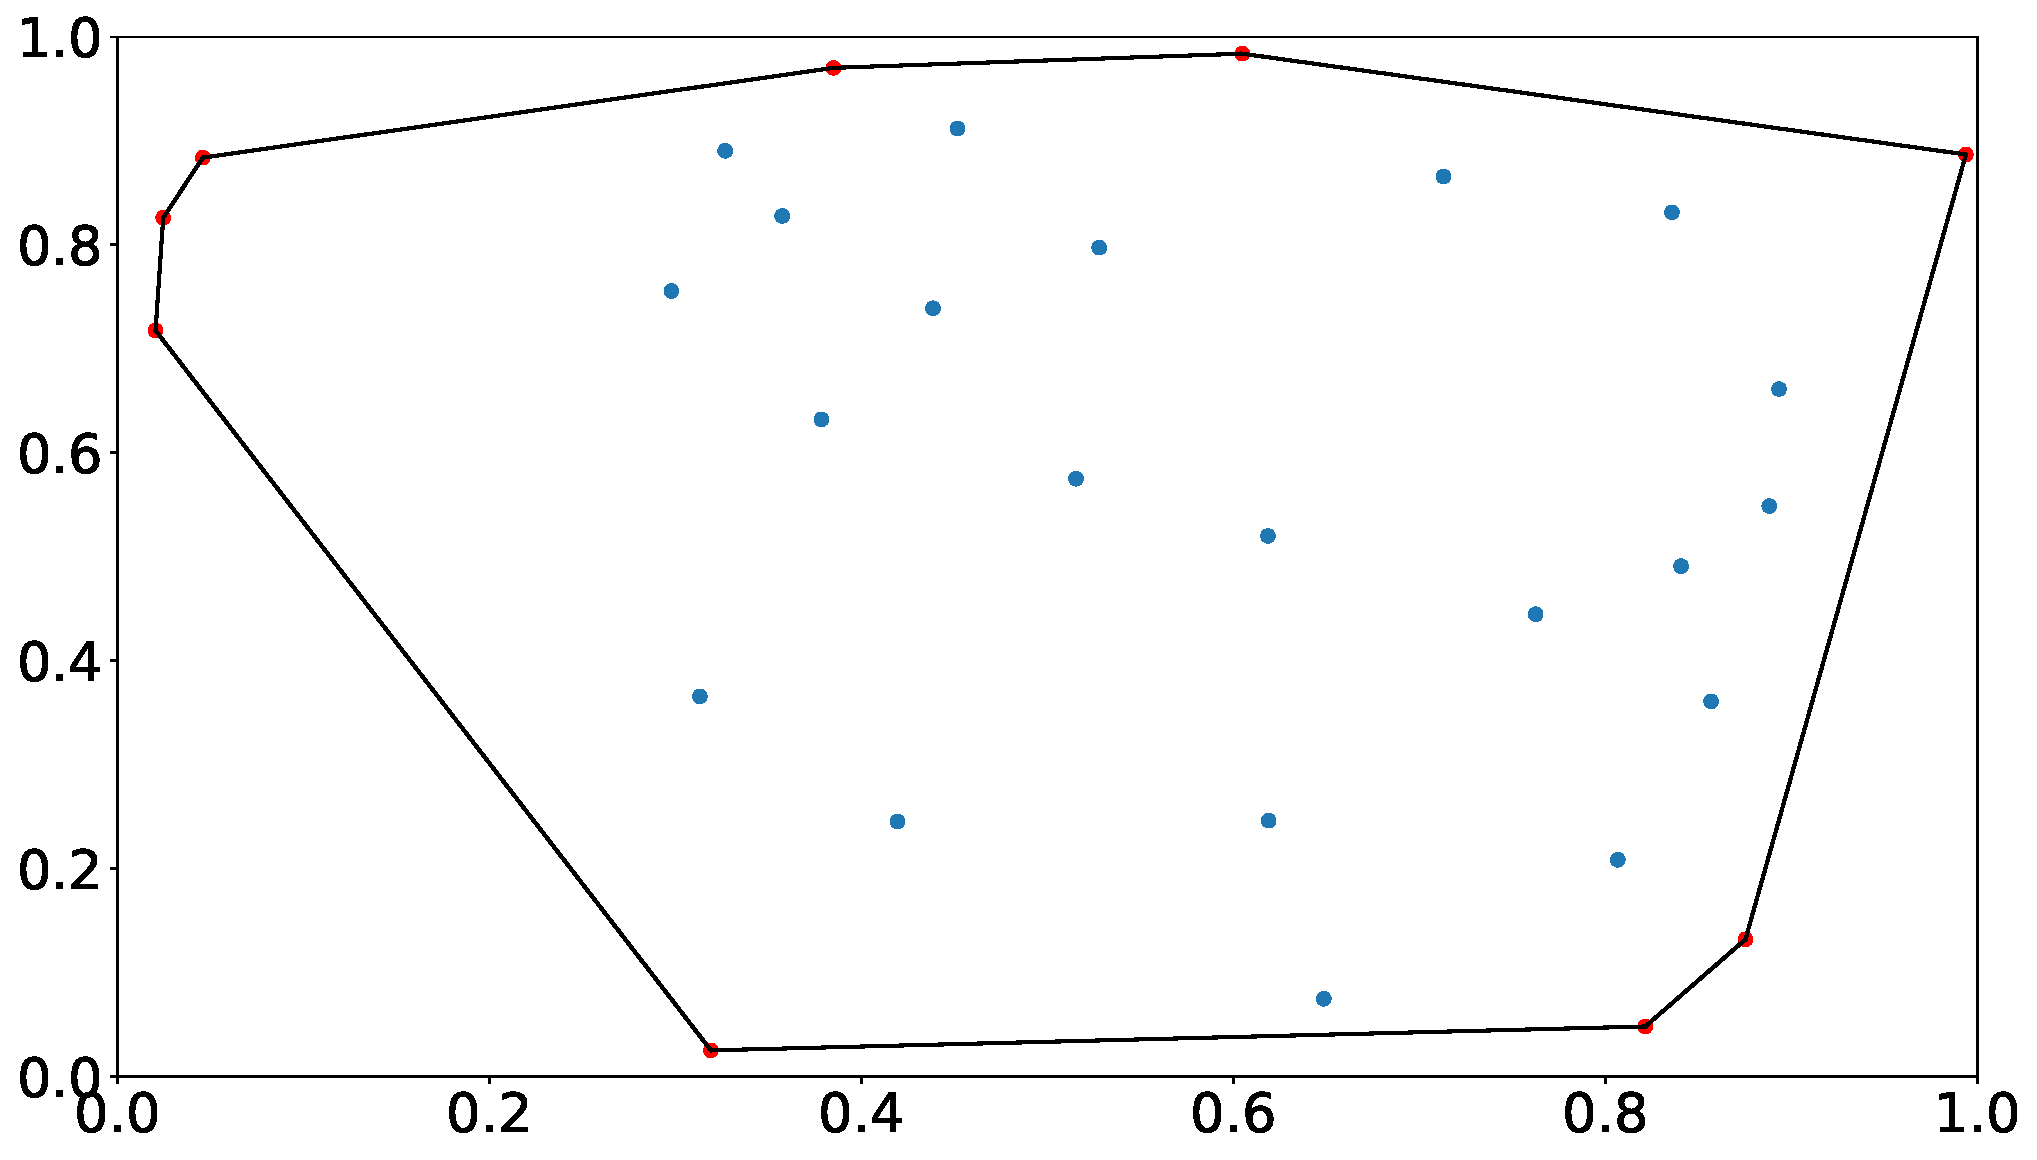
\includegraphics[width=\linewidth]{imgs/v-rep}
  \caption{Visualization of the V-representation of a set}%
  \label{fig:v-rep-example}
\end{figure}

A more useful representation of such regions is the \enquote{H-representation}.
In this representation, the intersection of a finite number of half-spaces
describes the region. A half-space is one of the two parts in which a
hyper-plane divides an affine space. Since half-spaces are linear inequalities,
the H-representation becomes the matrix inequality
%
\begin{equation}
  Ax\leq{}b,
\end{equation}
%
where \(A\) is a matrix of coefficients, \(x\) is a point in space and \(b\) is
a vector of real numbers. The number of rows in \(A\) and \(b\) is the same as
the number of half-spaces defining the region. All points satisfying the
inequality are in the region's interior, making it easy to test set membership.
Figure~\ref{fig:h-rep-example} shows the half-spaces that compose the
H-representation of the same convex polytope presented in
Figure~\ref{fig:v-rep-example}. Equation~\ref{eq:h-rep-example} shows the
inequation that describes the region. The selected side is not shown for each
half-space but is the one in which intersections with the other selected halves
make the convex region in the middle.

\begin{equation}
  \label{eq:h-rep-example}
  \begin{bmatrix}
    -0.91 & -0.39 \\
    0.04  & -0.99 \\
    0.98  & -0.15 \\
    0.84  & -0.54 \\
    -0.24 & 0.96  \\
    0.24  & 0.97  \\
    -0.06 & 0.99  \\
    -0.99 & 0.03  \\
    -0.93 & 0.34
  \end{bmatrix}x \leq
  \begin{bmatrix}
    -0.30 \\
    -0.01 \\
    0.84  \\
    0.66  \\
    0.84  \\
    1.10  \\
    0.94  \\
    0.00  \\
    0.26
  \end{bmatrix}
\end{equation}

\begin{figure}[!htb]
  \centering
  \includegraphics[width=\linewidth]{imgs/h-rep}
  \caption{Visualization of the H-representation of a set}%
  \label{fig:h-rep-example}
\end{figure}

Given that the V-representation is easier to obtain from generic shapes, but the
H-representation is more useful when verifying set membership, it is essential
to have a way to switch between them. Unfortunately, this is not
straightforward, but some algorithms allow us to enumerate the facets given the
vertices. Some problems of such algorithms are the time needed to find the
facets of many vertices and how to find facets in higher-order spaces. However,
good algorithms can be used for the conversion, especially if the computation
will be offline
\parencite{avis.bremner.ea:how,graham.frances-yao:finding,lee:on,mccallum.avis:linear}.

Particular regions can be easily described in a way that is easy to include in
optimization problems. The ellipsoid is one such region, as it is described as
\(x^{\top}Px\leq{}1\) so that any point \(x\) that satisfies the inequality is inside
the region. Any region described by polynomials can be expressed in a matrix
form and can quickly test membership. Such regions should use their inequation
directly instead of a polytope approximation. We do that to the Region of
Attraction, and it is how we implemented the check to verify if the state is
inside it.

\subsection{Internal Models}%
\label{subsec:internal-models}

To switch modes and controllers of a system the way we propose, one must pay
attention to the controller's internal states and the control signal's
continuity. Also, since every \CG{} unit has its controller and model, the
destination \CG{} must be updated to a valid state before switching. There are
many ways to do so, and we will present some.

One way is to run all \CG{}s in parallel. The optimization problem of the
inactive units does not need to run with complete constraints. It can be relaxed
only to contain the region constraint on the virtual reference; also, the
observer can be ignored. It is necessary to find the virtual reference, which
will be close to the constraint region's border, which is closest to the real
system's state. Notice that, in this case, we are not looking for a virtual
reference closest to the real reference but to the real system's state. By doing
so, the internal model's and the controller's states will always be valid.

However, this approach can be resource-intensive, as it still computes the
optimization problem at every sample. It is also possible to run the observer
and update the internal model's states without checking for constraint
violations, but this does not solve the controller's state problem. Another
technique needs to be combined to find them.

Another way of guaranteeing valid states is to compute the states before
changing mode. Two ways of computing the states are: by inverting the system and
controller equations and by simulation. The first approach has a very low
computational resource impact but may not be possible or yield not ideal values.
For systems with integrators, for example, there will be infinitely many
results. Another problem is that even though the system has only one
steady-state solution, it can have many transient ones.

The simulation becomes interesting, even though it is more computationally
intensive, as it can calculate a state that better matches the current
transitory characteristics of the real system. It can also find the model's and
controller's states at once, guaranteeing that there is no mismatch. To use the
simulation approach, execute the simulation right before changing modes, using
the internal controller and model, and setting the reference to the real
system's current state. This yields a valid steady-state model's and
controller's state. However, this technique does not guarantee control signal
continuity (which might even be impossible on some systems) without adjustments.

\subsection{Region of Attraction Estimation}%
\label{subsec:roa-estimation}

The Lyapunov approach presented in Section~\ref{subsec:region-of-attraction} can
easily estimate the region of attraction. The presented approach makes use of a
quadratic Lyapunov candidate, but it is not necessary, as it is possible to find
functions of any form. The function should easily to check if a point belongs to
the region, as it will be done frequently. Quadratic forms, such as the simple
one presented or those generated by Sum Of Squares techniques, are recommended
since they easily and computationally inexpensively check set membership.

The region of attraction needs to be larger than the constraints region and
needs to intersect all mode's regions of attraction to and from which it can
switch. Because of this, it is necessary to guarantee the intersection. However,
LMIs usually try to optimize the size of the region of attraction by making it
as big as possible or as small as possible. Since the exponential stability
tries to minimize the size of the region of attraction, we need a way to ensure
a minimum region size.

Consider the region of attraction described by
%
\begin{equation}
  x^{\top}Px \le{} 1,
\end{equation}
%
where \(x\) is the point that should be inside the region of attraction. (Note
that, numerically, a number smaller than \(1\) may be necessary to make the
problem feasible).

If the LMI is written in terms os \(P\), it can be used directly to force the
region to be big enough to contain the point \(x\). If the LMI is written in
terms of \(P^{-1}\), simply applying Schur's complement yields a valid LMI:
%
\begin{equation}
  \label{eq:lmi-point-inside-roa}
  \begin{bmatrix}
    P^{-1}   & x \\
    x^{\top} & 1
  \end{bmatrix} \succ \mathbf{0},
\end{equation}

You need to add one of such LMIs to your optimization problem for each mode that
is allowed to switch from or to the current mode. The point \(x\) does not need
to be the same for two modes that intersect, as placing the points some distance
apart creates a larger region of intersection, which gives a margin for errors.

To illustrate the choice of \(x\), consider the switched system composed of
three modes shown in Figure~\ref{fig:choice-x-roa-diff}. The stars represent
each mode's linearization point, the filled ellipses its constraints regions,
the unfilled circles the regions of attractions and the black dots the points
used in the LMIs to ensure the RoA's size. Note the intersection region formed
in the middle, displayed in yellow.

Now compare it with the same system, but only one point used for all systems,
depicted in Figure~\ref{fig:choice-x-roa-same}. See how smaller is the
intersection of regions of attraction and constraints (in yellow). The proposed
technique will be much more efficient in the first case, since it will result in
an earlier switch.

\begin{figure}[!htb]
  \centering
  \begin{subfigure}[b]{.45\linewidth}
    \centering
    \includesvg[width=\linewidth]{imgs/roa-choice-of-x-diff.svg}
    \caption{Choosing different \(x\) for each RoA}%
    \label{fig:choice-x-roa-diff}
  \end{subfigure}
  %
  \begin{subfigure}[b]{.45\linewidth}
    \centering
    \includesvg[width=\linewidth]{imgs/roa-choice-of-x-same.svg}
    \caption{Choosing the same \(x\) for all RoA}%
    \label{fig:choice-x-roa-same}
  \end{subfigure}
  \caption{Different RoA's intesections}%
  \label{fig:choices-of-x}
\end{figure}
